\chapter{The Problem and the Hardware}
\label{ch:problem}

While this system decodes tokens from a frontier-class model, its GPU rail
draws about $\sim$26\,W --- the chip barely warms. That is not efficiency;
it is a symptom. Each decode step at TP=2 must stream roughly
16.5--17\,GB of weights per rank through LPDDR5X memory that moves about
230--250\,GB/s in practice. At 250\,GB/s that is $\sim$68\,ms of mandatory
reading before any computation or communication happens. The GPU spends the
step waiting on memory, and that single piece of arithmetic shapes nearly
every design decision in this book.

Every serving system is shaped by one dominant constraint. In a hyperscaler
datacenter that constraint is usually cost per token at enormous scale; on
the system in this book it is far more concrete: \emph{how do you fit a
frontier mixture-of-experts model, a million-token KV cache, and a
speculative-decoding drafter into two desktop machines that share their GPU
memory with their operating system --- and still serve agents at interactive
speed?} This chapter establishes the mission, the hardware, and the physical
budgets that every later chapter negotiates with --- and resets the
datacenter instincts that would misjudge this platform twice before any
code is touched.

\section{The mission}
\label{sec:problem:mission}

The recipe's goal, stated in its own README, is to serve
\textbf{\code{deepseek-ai/DeepSeek-V4-Flash-Vision-Exp}} --- a
mixture-of-experts causal language model with multi-head latent attention
(MLA), a sparse attention indexer, native image input, and a built-in
speculative-decoding drafter called \textbf{DSpark}. The envelope below is
not a datasheet; it is a set of demands that collide --- a million-token
ceiling, times six concurrent sequences, inside 128\,GB of memory the
operating system also lives in:

\begin{itemize}
  \item a \textbf{1{,}048{,}576-token} (1M) per-request context ceiling;
  \item \textbf{six concurrent sequences}, aimed at agent workloads
    (long-lived coding and tool-use sessions, occasionally very deep);
  \item an OpenAI-compatible API on port 8888, complete with streaming, tool
    calling, reasoning control, and image input;
  \item \textbf{interactive decode speed}: roughly 62--83\,\tokspersec{} for a
    single stream, and 160--190\,\tokspersec{} aggregate across six short chats
    (measured August 2026; \Cref{ch:perf} discusses the later, lower band);
  \item multi-week uptime on hardware the operators own outright.
\end{itemize}

The serving engine is \textbf{vLLM} --- specifically a pinned, prebuilt fork
(the Anemll \repofile{dspark-vllm-gx10:0.1.1} image, examined in
\Cref{ch:architecture}) --- running \textbf{tensor parallelism of degree two
(TP=2)} across the two machines, with the model's own DSpark drafter
providing multi-token-prediction speculative decoding.

\begin{hbnote}
``1M context'' is a \emph{ceiling}, not a reservation. The KV pool is a
shared pool of about 2.33 million tokens on this build; any one request may
grow toward 1M, but six simultaneous full-1M requests cannot coexist ---
extras queue. \Cref{ch:profile} does this arithmetic in full.
\end{hbnote}

\section{The machine: NVIDIA DGX Spark}
\label{sec:problem:spark}

Every line of that envelope must be paid for out of a specific machine's
physical budgets, so the machine deserves a close reading before anything
else. A DGX Spark is a desktop machine built around the \textbf{GB10
Grace--Blackwell superchip}: a 20-core Arm Grace CPU and a Blackwell GPU
(compute capability \code{SM121}, targeted by kernels as \code{sm_121a}) that
share a single pool of \textbf{128\,GB unified LPDDR5X memory}. Each unit
also carries a \textbf{ConnectX-7} NIC whose 200\,Gb QSFP port --- a detail
that will matter greatly in \Cref{ch:fabric} --- enumerates as \emph{two}
PCIe Gen5~$\times$4 functions of roughly 126\,Gb/s each. \Cref{tab:problem:specs}
summarizes the platform as the repository's own audits observed it.

\begin{table}[htbp]
\centering\small
\caption{The serving platform, as observed live by the repository's audits
(September 2026).}
\label{tab:problem:specs}
\begin{tabular}{@{}l>{\raggedright\arraybackslash}p{5.6cm}>{\raggedright\arraybackslash}p{4.6cm}@{}}
\toprule
\textbf{Component} & \textbf{Per node} & \textbf{Consequence} \\
\midrule
CPU & 20-core Grace (Arm), performance governor & patch/orchestration side \\
GPU & Blackwell, SM121 (\code{sm_121a}) & consumer Blackwell kernel paths \\
Memory & 128\,GB unified LPDDR5X & GPU and OS share one pool \\
Mem.\ bandwidth & $\sim$230--250\,GB/s effective & \emph{the} decode constraint \\
NIC & ConnectX-7, 200\,Gb port as 2$\times$ Gen5 x4 PFs & fabric ceiling per PF \\
Software & CUDA 13.0, torch 2.11, driver 580.x & pinned in the image \\
Cluster & 2 nodes (default), optional 3rd & TP=2 default, TP=3 lane \\
\bottomrule
\end{tabular}
\end{table}

Two properties of this platform drive nearly every design decision in the
book, and they are worth internalizing now. One concerns who else is
spending the memory; the other concerns how quickly that memory can be
read. Both reduce to arithmetic the later chapters keep re-deriving.

\subsection{Unified memory: the OS lives inside your GPU budget}
\label{sec:problem:unified}

On a datacenter GPU, host RAM and HBM are separate worlds; an OS daemon
leaking memory cannot evict your KV cache. On GB10 they are the same
128\,GB. The consequence is that \emph{host-side} memory pressure is a
\emph{GPU-side} serving hazard:

\begin{itemize}
  \item vLLM's \code{--gpu-memory-utilization} budget (0.835 here) governs
    weights plus KV pool, but activation workspaces, JIT compiler caches,
    NCCL buffers, and every host process draw from the same physical pool
    \emph{outside} that budget;
  \item two prefill-tuning experiments that were perfectly sound as GPU
    changes were \emph{rejected purely on host memory}: raising the prefill
    chunk cap cost 1.5\,GB of head-node \code{MemAvailable} and started
    swap growth (\Cref{ch:perf}).
\end{itemize}

The repository's September 2026 audit caught this hazard live. Both nodes
were exhausting memory at boot --- kernel logs full of
\code{NV_ERR_NO_MEMORY}, 10.4\,GB of swap in use on the worker. The cause
was pure desktop software on a headless serving node: a 3.1\,GB
\code{polkitd} leak and a GNOME session (Xorg plus gnome-shell) still
holding GPU contexts.

Because vLLM sizes the KV pool from the \emph{minimum} across ranks, the
worker's bloat was costing cache on both nodes. The audit ranked reclaiming
that memory --- an estimated 5--8\,GB, worth +20--35\,\% KV tokens at a
raised utilization --- the single highest-value fix available
(\Cref{ch:perf}). The follow-up confirmed it: switching the worker to
\code{multi-user.target} zeroed its swap and evicted the leak (and promptly
surfaced the next one, a 3.8\,GB \code{wireplumber} process). A desktop
daemon had been quietly shrinking a frontier model's KV pool. Generalized:
on unified memory the KV pool is a residual --- whatever the two operating
systems have not already spent --- so capacity work starts with host
hygiene rather than with the engine's flags. \Cref{fig:problem:pool} shows
who else is spending the pool.

\begin{figure}[htbp]
\centering
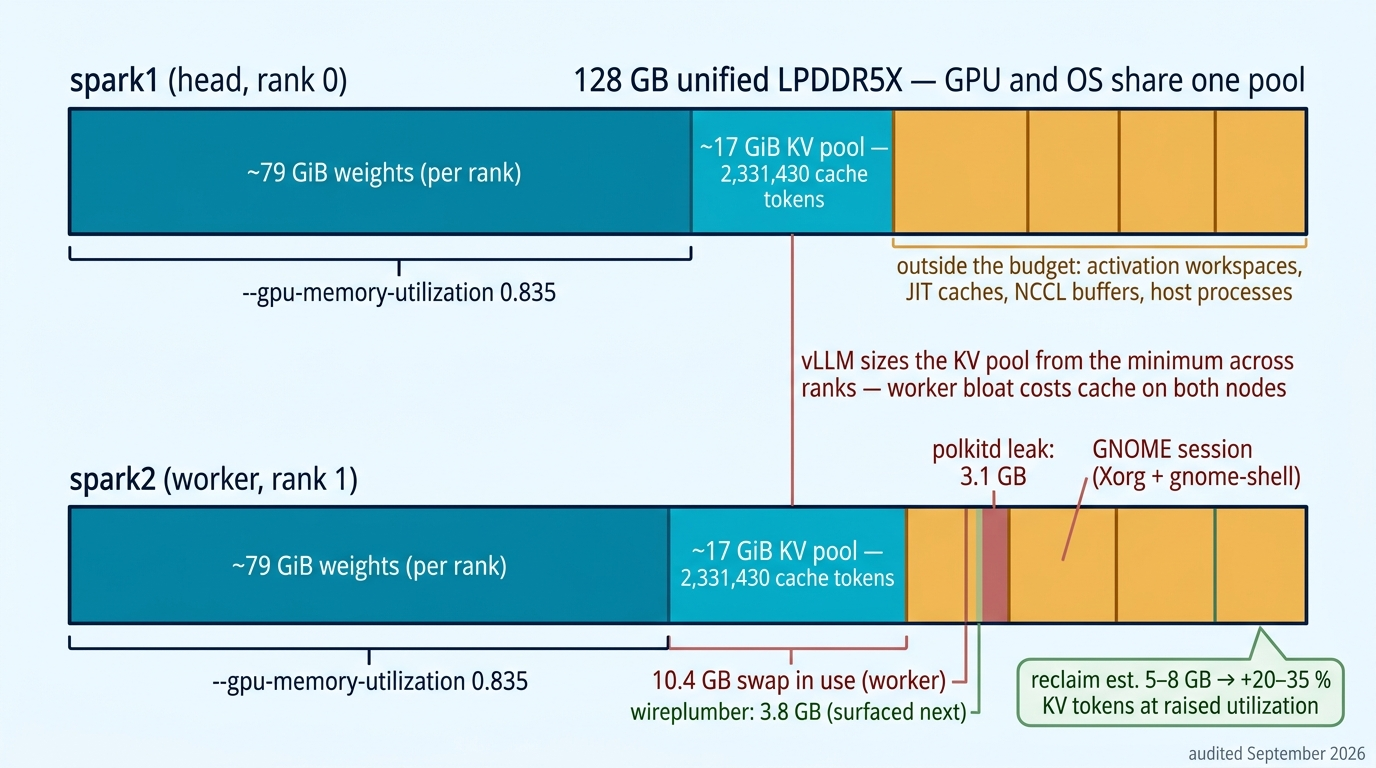
\includegraphics[width=\textwidth]{figures/ch01-128gb-pool.png}
\caption{Unified memory as a contested budget. The utilization target
governs only weights plus KV pool; activation workspaces, JIT caches, NCCL
buffers and every host process spend the same 128\,GB from outside it.
Because vLLM sizes the pool from the \emph{minimum} across ranks, the
worker's 3.1\,GB \code{polkitd} leak and desktop session were shrinking the
KV cache on both nodes (September 2026 audit).}
\label{fig:problem:pool}
\end{figure}

\begin{hbwarning}
The stock \code{earlyoom} daemon on DGX Spark hosts \emph{can} kill vLLM under
deep-context load --- the repository's quick start instructs disabling it on
both hosts. On unified memory, an out-of-memory killer
tuned for desktops is pointed straight at your inference engine.
\end{hbwarning}

\subsection{Bandwidth: decode is a streaming problem}
\label{sec:problem:bandwidth}

Sharing the pool is only half of the platform's tax; the other half is how
slowly the pool moves. LPDDR5X moves roughly 230--250\,GB/s in practice --- an order of magnitude
below datacenter HBM. The 16.5--17\,GB each rank must stream per decode
step is dominated by the touched subset of 256 routed experts across 43
layers, plus attention weights, the drafter, and the language-model head
(\Cref{ch:perf} derives the budget line by line). The arithmetic from the
opening page turns those bytes into $\sim$68\,ms of mandatory reading: a
single stream simply cannot exceed a few dozen steps per second, no matter
how clever the kernels are. Everything that makes this system fast follows
from that arithmetic:

\begin{itemize}
  \item \textbf{speculative decoding} (DSpark, \Cref{ch:specdecode}) makes
    each expensive step emit $\sim$3--4 accepted tokens instead of one;
  \item \textbf{concurrency} amortizes the same weight stream across six
    requests, which is why c=6 aggregate throughput is $\sim$2.2$\times$ a
    single stream;
  \item \textbf{quantization} (FP8 weights, MXFP4 experts, FP8-enveloped KV)
    shrinks the bytes that must move.
\end{itemize}

One lever conspicuously fails: a third machine \emph{does not} speed up a
single stream. The TP=3 experiment cut bytes per rank by a third yet
decoded no faster, because fixed per-step costs --- about 108 NCCL
collectives per decode step --- filled the gap. More hardware is not a
lever here, and \Cref{ch:scaling} proves it the hard way.
\Cref{fig:problem:bytes} puts the bytes, the reading floor, and the three
levers on one page.

\begin{figure}[htbp]
\centering
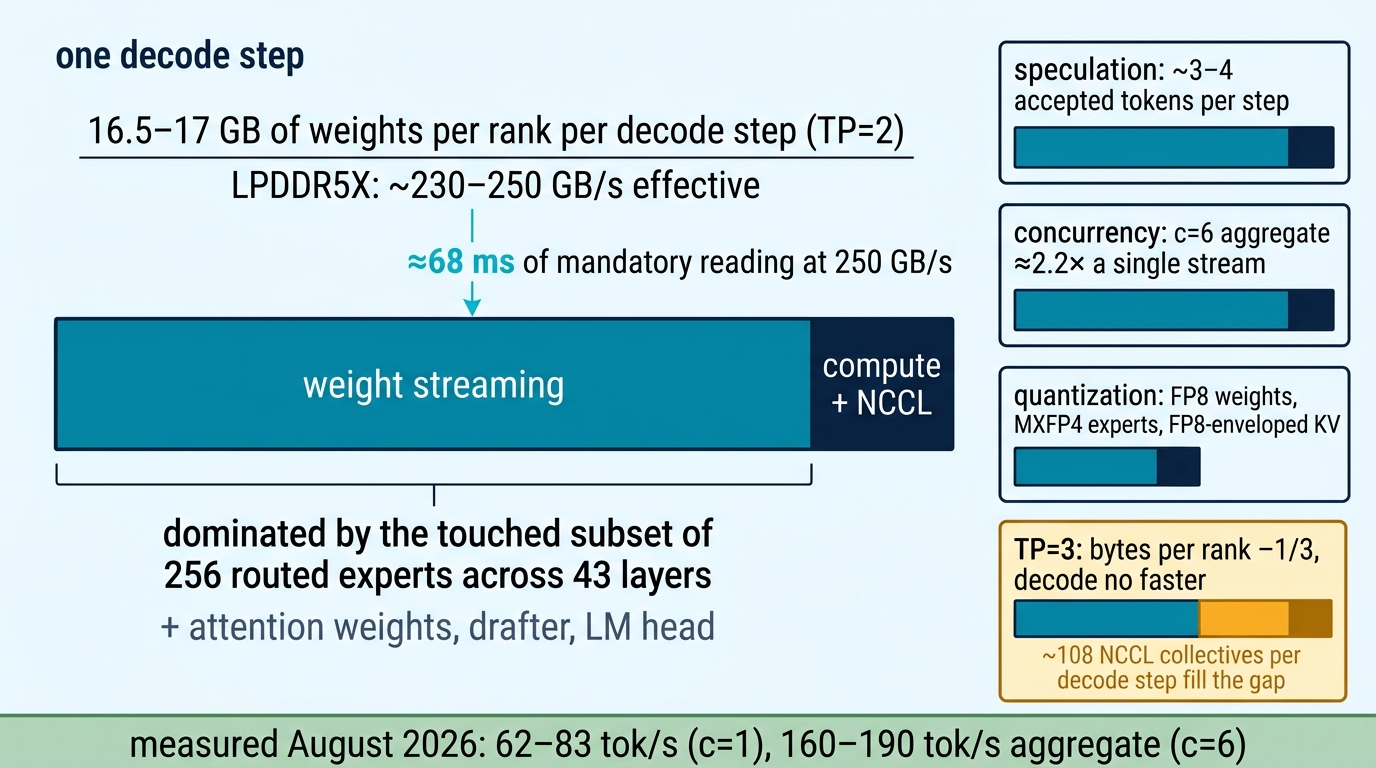
\includegraphics[width=\textwidth]{figures/ch01-decode-step-bytes.png}
\caption{Decode as a streaming problem. Each step must read
16.5--17\,GB of weights per rank through 230--250\,GB/s of LPDDR5X ---
68--74\,ms of mandatory reading before any compute or collective. Only
levers that change the bytes (quantization) or the accepted tokens per step
(speculation, concurrency) move the result; a third machine shrinks the
bytes but refunds the saving in fixed per-step collectives.}
\label{fig:problem:bytes}
\end{figure}

\begin{hblesson}
Before tuning anything, write down the bytes your decode step must stream
and divide by your measured memory bandwidth. If the answer is close to your
observed step time, you are streaming-bound: only fewer bytes per accepted
token (quantization, better draft acceptance) or more tokens per step
(concurrency, speculation) can help. Kernel micro-optimizations cannot.
\end{hblesson}

\section{Two machines, one engine}
\label{sec:problem:twonodes}

The byte budget claims its first casualty before a single request arrives.
The FP8 checkpoint is roughly 157\,GB --- it does not fit in one 128\,GB
node alongside a useful KV cache. The model is therefore sharded with tensor
parallelism across the pair: every layer's weights are split between the two
GPUs, and every decode step synchronizes them over the RoCE link. At TP=2
each rank holds $\sim$79\,GiB of weights, leaving about \textbf{17\,GiB of
KV pool} per rank at the default utilization --- 2{,}331{,}430 cache tokens,
which is what makes the 1M ceiling with multi-session concurrency workable.
Tensor parallelism is doing capacity work here rather than speed work: the
second machine buys the memory to hold the checkpoint, and every decode step
pays for that purchase in synchronization.

\Cref{fig:problem:topology} shows the physical arrangement. One node is the
\emph{head}: it runs rank~0, serves the HTTP API, and orchestrates
everything. The other is the \emph{worker}: rank~1, headless, reached by the
head over SSH for lifecycle operations and over the ConnectX fabric for
NCCL collectives, TCP bootstrap, the scheduler's ZeroMQ broadcasts, and
(optionally) NFS-shared model weights.

\begin{figure}[htbp]
\centering
\begin{tikzpicture}[node distance=6mm and 10mm]
  % Head node
  \node[hbhost, minimum width=52mm, minimum height=42mm] (head) {};
  \node[hbtitle, anchor=north] at ($(head.north)+(0,-1.5mm)$) {spark1 (head, rank 0)};
  \node[hbnode, below=7mm of head.north, minimum width=40mm] (hcpu) {Grace CPU\\\scriptsize launcher, Docker, API};
  \node[hbgpu, below=3mm of hcpu, minimum width=40mm] (hgpu) {Blackwell GPU\\\scriptsize 79 GiB weights + 17 GiB KV};
  \node[hbfaint, below=3mm of hgpu, minimum width=40mm, minimum height=7mm] (hmem) {\scriptsize 128 GB unified LPDDR5X};
  % Worker node
  \node[hbhost, minimum width=52mm, minimum height=42mm, right=34mm of head] (wrk) {};
  \node[hbtitle, anchor=north] at ($(wrk.north)+(0,-1.5mm)$) {spark2 (worker, rank 1)};
  \node[hbnode, below=7mm of wrk.north, minimum width=40mm] (wcpu) {Grace CPU\\\scriptsize headless container};
  \node[hbgpu, below=3mm of wcpu, minimum width=40mm] (wgpu) {Blackwell GPU\\\scriptsize 79 GiB weights + 15--17 GiB KV};
  \node[hbfaint, below=3mm of wgpu, minimum width=40mm, minimum height=7mm] (wmem) {\scriptsize 128 GB unified LPDDR5X};
  % NICs
  \node[hbbox, below=4mm of head, minimum width=40mm] (hnic) {ConnectX-7\\\scriptsize 2 PFs, Gen5 x4 each};
  \node[hbbox, below=4mm of wrk, minimum width=40mm] (wnic) {ConnectX-7\\\scriptsize 2 PFs, Gen5 x4 each};
  \draw[hbflow, very thick] (hnic) -- node[hblabel, above]{200 Gb QSFP (RoCE v2)}
    node[hblabel, below]{NCCL / bootstrap / ZMQ / NFS} (wnic);
  % LAN
  \node[hbfaint, below=9mm of $(hnic.south)!0.5!(wnic.south)$, minimum width=60mm, minimum height=6mm] (lan) {\scriptsize LAN (RJ45): SSH control plane, clients};
  \draw[hbarrow, dashed] (hnic.south) to[out=-90,in=90] (lan.north west);
  \draw[hbarrow, dashed] (wnic.south) to[out=-90,in=90] (lan.north east);
  % Client
  \node[hbnode, left=9mm of head, minimum width=16mm] (client) {clients\\\scriptsize :8888};
  \draw[hbarrow] (client) -- (head.west);
\end{tikzpicture}
\caption{The two-node serving cluster. The model is sharded TP=2 across the
GPUs; every decode step synchronizes over the direct 200\,Gb RoCE link, while
lifecycle control (SSH) and client traffic ride the ordinary LAN.}
\label{fig:problem:topology}
\end{figure}

Splitting one engine across two commodity hosts buys the memory the model
needs, but it also buys a distributed-systems tax that recurs throughout
this book: the pair fails \emph{as a pair}. A rank stalled in a mid-serve
JIT compilation leaves its peer blocked in a collective until the torch NCCL
watchdog kills it after 600 seconds (\ghissue{117}). A reboot can resurrect
one rank but not the other. A patch applied to one writable container layer
but not the other produces divergent engines. Much of the operational
discipline in \Cref{ch:patches,ch:operations} exists precisely to keep two
loosely coupled machines behaving like one engine.

\section{The economics, briefly}
\label{sec:problem:econ}

After a chapter spent pricing constraints --- shared memory,
streaming-bound decode, a pair that fails as a pair --- it is worth naming
what they buy: why this configuration is interesting beyond its own
walls. Two DGX Sparks cost on the order of a used car, sit under a desk, and
draw the modest power that opened this chapter. For that, the operators get a private frontier-class model with a million
tokens of context, native vision, tool calling, and $\sim$190\,\tokspersec{}
aggregate throughput --- enough to run a small team's agents with no per-token
bill and no data leaving the room. The price is paid in engineering instead:
the roughly forty runtime patches, the measurement rigs, and the operational
doctrine that the rest of this handbook documents. Whether that trade is
right for any given team is situational; what this system demonstrates is
that the trade is \emph{available}, and what it actually costs.

\FloatBarrier
The 26 watts on the opening page are no longer a puzzle. A decode step on
this cluster is not a computation with a memory cost; it is a memory read
--- 16.5--17\,GB per rank through 230--250\,GB/s, 68--74\,ms of it ---
with a computation attached, and the second machine is there to hold the
checkpoint rather than to go faster. The 128\,GB is not a GPU budget either:
it is a budget two operating systems are already spending from, which makes
the KV pool a residual rather than an allocation.

\section*{Takeaways}
\begin{itemize}
  \item The mission: DeepSeek-V4-Flash (MoE + MLA + sparse indexer + DSpark
    drafter + vision) at a 1M-token ceiling and six concurrent agent
    sessions, on two GB10 DGX Sparks with vLLM at TP=2 --- where the second
    machine buys the memory for a $\sim$157\,GB checkpoint, not speed, and
    every decode step pays for that purchase in synchronization.
  \item Unified memory makes host RAM part of the GPU budget: OS daemons,
    JIT caches, activation workspaces and NCCL buffers spend the same
    128\,GB from \emph{outside} the utilization target, an OOM killer tuned
    for desktops targets the engine, and because vLLM sizes the pool from
    the minimum across ranks, one node's leak shrinks the cache on both.
    Capacity work therefore starts with host hygiene --- the audit put the
    reclaimable 5--8\,GB at +20--35\,\% KV tokens at a raised utilization.
  \item Decode is weight-streaming-bound: only fewer bytes per accepted
    token (quantization, better acceptance) or more tokens per step
    (speculation, concurrency) move it at c=1. A third machine does not:
    TP=3 cut bytes per rank by a third and decoded no faster, because the
    $\sim$108 fixed collectives per step refunded the saving.
  \item A TP pair fails as a pair: a rank stalled in mid-serve JIT leaves
    its peer blocked until the 600-second NCCL watchdog fires
    (\ghissue{117}), reboots can resurrect one rank and not the other, and
    a patch applied to one container layer produces divergent engines ---
    the pair-level hazards that shape the operational doctrine of later
    chapters.
\end{itemize}

\chaptertransition{Constraints this tight leave no room for an engine you
cannot account for. If the KV pool is whatever two operating systems have
not already spent, and if the two machines fail as a unit, then ``which
bytes are actually running, on both ranks?'' stops being a hygiene question
and becomes a capacity and reliability question --- one that has to be
answered by construction rather than by inspection after the fact. The next
chapter opens a stack whose answer is deliberately strange: about forty
source patches applied to the inference engine at every container start,
each chained with \code{|| exit 1}, on top of a prebuilt image the
repository refuses to rebuild. A serving stack built to fail its own boot
--- why would anyone run a frontier model that way?}
